\documentclass[times, utf8, seminar, numeric]{fer}
\usepackage{booktabs}
 \usepackage{url}
\usepackage{graphicx}
\usepackage{float}
\begin{document}

% Ukljuci literaturu u seminar
\nocite{*}

% TODO: Navedite naslov rada.
\title{Vlastita implementacija filtera: \protect\\ The Logarithmic Dynamic Cuckoo Filter}

% TODO: Navedite vaše ime i prezime.
\author{Fran Ostroški, Elena Wachtler}

% TODO: Navedite ime i prezime voditelja.
\voditelj{Mirjana Domazet-Lošo}

\maketitle

\tableofcontents

\chapter{Uvod}

Ovaj seminar opis je projekta u sklopu kolegija Bioinformatika 1 Fakulteta elektrotehnike i računarstva Sveučilišta u Zagrebu, a predstavlja vlastitu implementaciju takozvanog cuckoo filtera, točnije njegovu dinamičku logaritamsku varijantu. \\

Cuckoo filter probabilistička je struktura podataka koja se koristi za određivanje pripadnosti zadanog elementa nekome skupu. Sam filter nastao je kao proširenje već postojećih Bloom filtera, a naziv je dobio prema ptici kukavici koja izbacuje jaja iz tuđih gnijezda kako bi ubacila svoja. Iako je riječ o općenitim podatcima, cuckoo filter često se primjenjuje u bioinformatici jer je pogodan za određivanje pripadnosti podnizova nukleotidnih slijedova nekom većem nizu nukleotida ili provjeru nalaze li se podnizovi jednog slijeda u nekom drugom slijedu.

Pripadnost elementa nekom skupu ovom strukturom ne možemo garantirati, jer zbog implementacije algoritma postoji malena vjerojatnost za lažno pozitivne (eng. \textit{false positive}) i lažno negativne (eng. \textit{false negative}) rezultate. Upravo zbog toga što postoji određena vjerojatnost pogreške, cuckoo filter je probabilistički. Međutim, nepripadnost nekom skupu može se pouzdano odrediti. \\


\chapter{Opis algoritma}

\begin{flushleft}
\textbf{Nastanak i evolucija Cuckoo filtera}
\end{flushleft}

Cuckoo filtere kao ideju za rješavanje problema koji zahtjevaju nisku stopu lažno pozitivnih primjera predstavili su Fan, Kaminsky i Andersen \cite{DBLP:journals/usenix-login/FanAK13}, kao strukturu čija je glavna prednost u odnosu na dotad korištene Bloom filtere sposobnost brisanja. Čak štoviše, uvode cuckoo filtere kao strukturu koja ne samo da omogućuje dinamičko dodavanje i brisanje objekata, već postiže bolje \textit{lookup} performanse, pri tome koristeći manje prostora od dotad optimalnih Bloom filtera.
Teoriju koju su predložili kasnije su i dokazali \cite{10.1145/2674005.2674994} - cuckoo filteri uistinu su nadmoćna struktura za pohranu velikog broja objekata, kada je nužan uvjet niska stopa lažno pozitivnih primjera. Uz to, dodana su i poboljšanja kako bi se smanjila prostorna složenost, i to djelomičnim sortiranjem bucketa te optimizacijom veličine bucketa - najboljim se pokazao (2, 4)-cuckoo filter, što znači da svaki objekt ima dva moguća kandidata za bucket, a svaki bucket u sebi sadrži podatke o četiri otiska (eng. \textit{fingerprint}). O bucketima je više rečeno u nastavku poglavlja gdje je dan detaljan opis rada algoritma uz primjer.

Korak dalje učinili su Chen, Liao, Jin i Wu \cite{8117563} uvođenjem dinamičkog cuckoo filtera, koji bi istovremeno zadovoljavao i uvjet da se veličina strukture može fleksibilno mijenjati, ali i da operacija brisanja bude pouzdana. Autori tvrde da ovakva implementacija cuckoo filtera koja u sebi sadrži povezanu listu filtera ostvaruje 75\% smanjeno zauzeće memorije, poboljšanje u konstrukciji strukture od 50\% te ubrzanje u operaciji \textit{query} od čak 80\%. Također, kao dodatnu optimizaciju uvode gornje ograničenje na broj relokacija. Relociranje je vizualizirano u nastavku poglavlja gdje je algoritam primijenjen na jednostavan primjer.

Posljednju nadogradnju ostvarili su Zhang, Chen, Jin i Reviriego \cite{9458864} ističući linearno rastuću računalnu i prostornu složenost s rastom veličine prostora podataka kao glavni nedostatak dinamičkih cuckoo filtera, te uvodeći višerazinsko binarno stablo kao rješenje tog nedostatka, zbog čega se njihova struktura naziva logaritamskim dinamičkim cuckoo filterom, LDCF. S ovim poboljšanjem, operacije dodavanja novih objekata i provjera nalazi li se objekt u strukturi (eng. \textit{membership testing}) od složenosti \textit{O(N)} (gdje je \textit{N} veličina skupa podataka) padaju na složenost \textit{O(1)}. Dodatno, ponudili su i varijantu kompaktnog LDCF-a u kojoj je dodatno smanjeno prostorno zauzeće, na način da se zadržava samo najviša razina cuckoo filtera u višerazinskom stablu. U ovome radu u poglavlju \ref{Analiza} analizirane su performanse vlastite implementacije upravo ove, najviše unaprijeđene varijante cuckoo filera - LDCF.




\begin{flushleft}
\textbf{Vizualizacija algoritma na jednostavnom primjeru}
\end{flushleft}


U općenitom slučaju, cuckoo filter sastoji se od nizova memorijskih lokacija koje se nazivaju \textit{bucketima}. Bucketi mogu imati mjesta za više unosa, ali u ovom jednostavnom primjeru svaki bucket moći će primiti  po jedan uneseni podatak.

Neka je dan jedan kratak nukleotidni slijed, npr. AACTGAT, te se kao ulazi u filter trebaju unijeti svi njegovi k-meri, za k = 3. To su : AAC, ACT, CTG, TGA i GAT . \\
U prvom koraku algoritma za svaki unos računaju se dva sažetka (eng. \textit{hash}) pomoću odabranih funkcija sažimanja (tzv. \textit{hash} funkcija).

\begin{figure}[H]
  \centering
  \setlength{\intextsep}{5pt}
  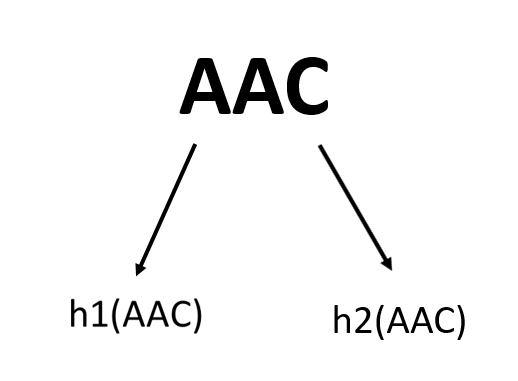
\includegraphics[scale = 0.75]{images/hashing.png}
  \caption{Generiranje hasha - Fran Ostroški}
  \label{fig_hash}
\end{figure}

U drugom se koraku iz generiranih sažetaka određuje indeks bucketa u koji će biti smješten ulazni niz. To se najčešće određuje uporabom operacije dijeljenja \textit{modulo} s ukupnim brojem bucketa. Kada se generiaju oba indeksa, element će se spremiti na jedno od dvije lokacije s tim indeksima. Svrha drugog sažetka je smanjenje vjerojatnosti kolizije i potrebe za premještanjem. Drugi sažetak ovisi i o trenutnoj poziciji elementa kako bi se osiguralo da se alternative razlikuju. 


\begin{figure}[H]
  \centering
  \setlength{\intextsep}{5pt}
  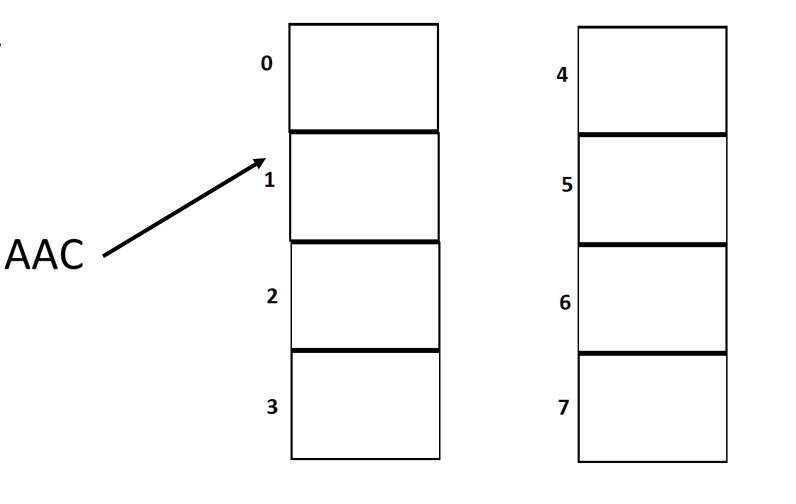
\includegraphics[scale = 0.4]{images/insertion1.png}
  \caption{Odabir lokacije za niz AAC - prikaz po uzoru na [2]}
  \label{fig_insert1}
\end{figure}
Idući je na redu niz ACT. Nakon generiranja sažetaka smješta se u prazni bucket. Ovdje još uvijek nema kolizija.
\begin{figure}[H]
  \centering
  \setlength{\intextsep}{5pt}
  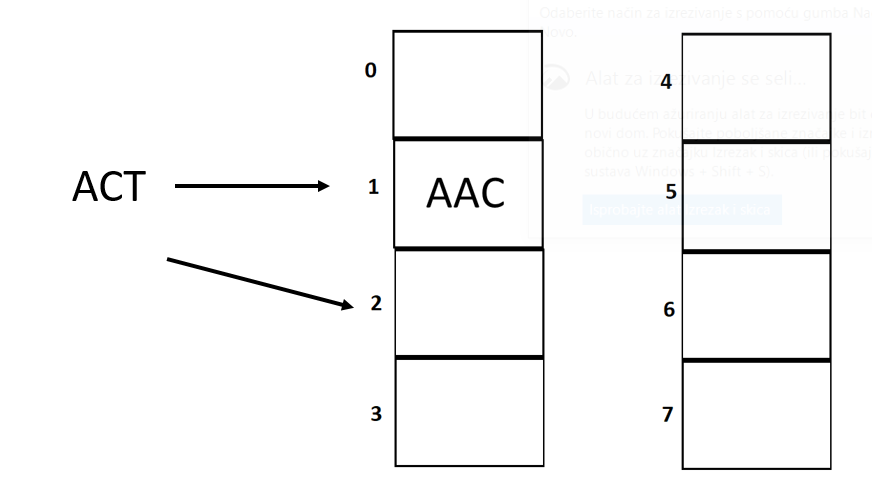
\includegraphics[scale = 0.4]{images/insertion2.png}
  \caption{Odabir lokacije za niz ACT - prikaz po uzoru na [2]}
  \label{fig_insert2}
\end{figure}
Za niz CTG dogodila se situacija da je lokacija na koju ga želimo pohraniti već popunjena. Tada se u algoritmu događa "izbacivanje". Obabrani se element izbacuje, umeće se CTG, a za izbačeni element traži se nova lokacija.Novu lokaciju za izbačeni element dobivamo pomoću izračunat h2(CTG).

\begin{figure}[H]
  \centering
  \setlength{\intextsep}{5pt}
  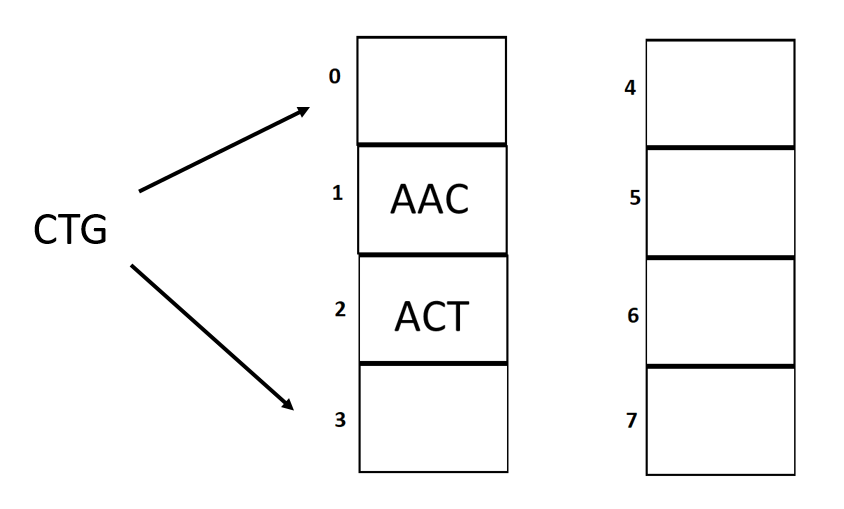
\includegraphics[scale = 0.4]{images/insertion3.png}
  \caption{Odabir lokacije za niz CTG - prikaz po uzoru na [2]}
  \label{fig_insert3}
\end{figure}

Za niz TGA dogodila se  ista situacija. Za element AAC pomoću h2(AAC) računa se alternativna adresa na koju se pohranjuje.

\begin{figure}[H]
  \centering
  \setlength{\intextsep}{5pt}
  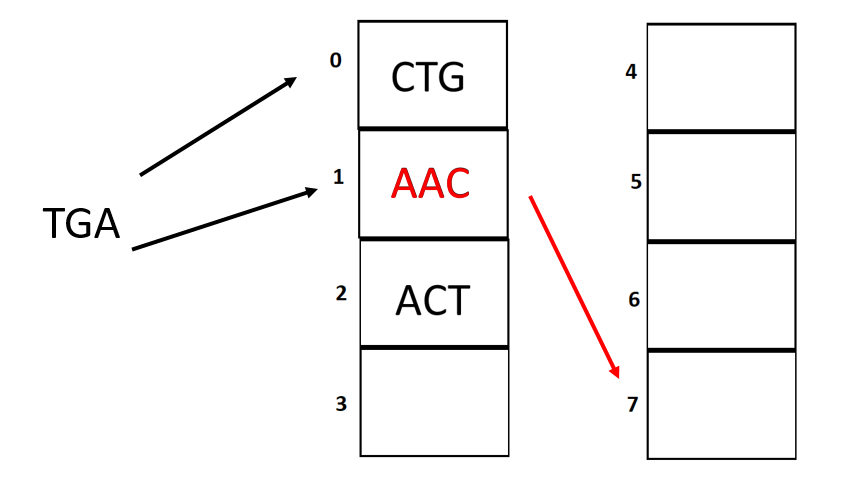
\includegraphics[scale = 0.4]{images/swap1.png}
  \caption{Izbacivanje AAC i ubacivanje TGA - prikaz po uzoru na [2]}
  \label{fig_swap1}
\end{figure}

Za niz GAT također se mora izvršiti izbacivanje starog elementa. Međutim, sada je i adresa na koju bi TGA bio premješten već popunjena. Tada se za element ACT ponovno računa nova pozicija koja zbog korištenja trenutnog indeksa u izračunu neće biti identična. 

\begin{figure}[H]
  \centering
  \setlength{\intextsep}{5pt}
  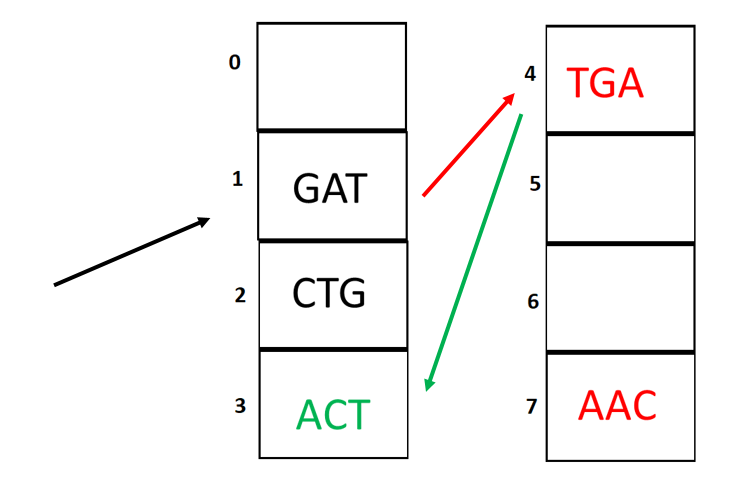
\includegraphics[scale = 0.4]{images/swap2.png}
  \caption{Izbacivanje TGA i ubacivanje GAT, relociranje ACT - prikaz po uzoru na [2]}
  \label{fig_swap2}
\end{figure}

\begin{figure}[H]
  \centering
  \setlength{\intextsep}{5pt}
  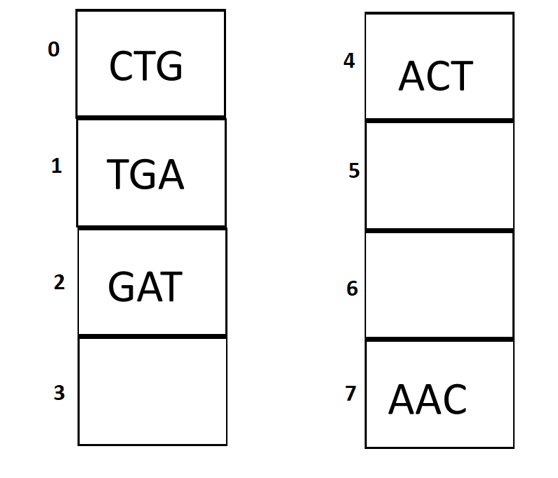
\includegraphics[scale = 0.4]{images/finalalign.png}
  \caption{Konačni razmještaj elemenata - prikaz po uzoru na [2]}
  \label{fig_finalalign}
\end{figure}

Može se primijetiti da što je popunjenost veća, raste i vjerojatnost da će doći do izbacivanja i relokacije starijih elemenata u filteru. Dogodit će se situacije da će element koji se premješta biti premješten na već popunjeni bucket. U tom slučaju prijašnji element će se premjestiti, te će postupak nastaviti sve dok se ne pronađe slobodno mjesto ili se dosegne maksimalan broj operacija premještanja. U slučaju da se dosegne maksimalan broj, to je obično indikator skore popunjenosti filtera. U tom slučaju mogu se poduzeti razne akcije, koje su ponovno različite za svaku implementaciju filtera. \\



\begin{flushleft}
\textbf{Dodatak opisa rada LDCF}
\end{flushleft}



Algoritam LDCF započinje samo jednim CF-om, koji smatramo da je nulta razina budućeg višerazinskog stabla. Pri tome se element dodaje u CF tako da se njegov ranije spomenuti otisak (eng. \textit{fingerprint}) dodaje u bucket. Jednom kada se dogodi da operacija \textit{insert} ne uspije, smatra se da je CF pun, te se dodaju dva nova CF-a. Kada se dodaje novi objekt u jedan od dva nova CF-a, promatra se prvi bit njegova fingerprinta, te prema tome određuje hoće li biti smješten u lijevi novododani CF, za vrijednost prvog bita fingerprinta jednaku nula, ili desni novododani CF, za slučaj kada je prvi bit njegova fingerprinta jednak jedan. Budući da je time vrijednost prvog bita implicitno zapisana u poziciji elementa u stablu, taj se bit uklanja iz fingerprinta i fingerprint se pohranjuje bez njega. Taj se postupak dalje propagira na niže razine.

Jedna od glavnih prednosti algoritma LDCF nad DCF jest velika mogućnost paralelizacije. Naime, u DCF-u sve operacije \textit{insert} izvode se na istom CF-u, dok su u LDCF-u grane s CF-ima međusobno neovisne zbog opisanog načina kako se konstruiraju, te se zbog toga operacije \textit{insert} mogu izvoditi istovremeno na neovisnim granama.


\begin{flushleft}
\textbf{O implementaciji}
\end{flushleft}

Za implementaciju je korišten programski jezik C++. Ulazni podatci učitavaju se iz datoteke i rezultati se ispisuju u vanjsku izlaznu datoteku. Što se tiče vanjskih knjižnica, korišten je OpenSSL, knjižnica koja je uključena u bio-linux.

Prijašnji radovi \cite{10.1145/3485983.3494852} sugeriraju da je četiri unosa po bucketu optimalna veličina bucketa, ali u ovoj je konkretnoj implementaciji odabrana konfiguracija s bucketom koji prihvaća maksimalno osam unosa. Tesitiranjem različitih varijacija, zaključeno je da je za takvu  implementaciju optimalna manja veličina cuckoo filtera od onih koje predlažu drugi radovi - manji broj bucketa po cuckoo filteru - konkretno, u testovima navedenima u analizi, korišteni su cuckoo filteri koji sadrže šesnaest bucketa.
 
\chapter{Analiza}
\label{Analiza}

U tekstu koji slijedi dana je analiza točnosti, vremena izvođenja i utroška memorije za različite testne slučajeve. Testovi su izvođeni u nekoliko inačica, koristeći:
\begin{itemize}

  \item {sintetske podatke - nizovi duljine od $10^3$ do $10^7$ znakova}
  \item {stvarne podatke - genom bakterije Escherichia coli.}

\end{itemize}


\begin{flushleft}
\textbf{Analiza na sintetskim podatcima}
\end{flushleft}

\begin{tabular}
{ |p{0.8cm}||p{4cm}|p{4cm}|p{4cm}|  }
 \hline
 \multicolumn{4}{|c|}{Ručno generirani nukleotidni sljedovi} \\
 \hline
 r. br. testa& vrijeme izvođenja operacije insert \textit{(s)} & vrijeme izvođenja operacije query \textit{(s)} &zauzeće memorije \textit{(MB)}\\
 \hline
 1& AF    &AFG&   004\\
 2&   AX  & ALA   &248\\
 3&AL & ALB&  008\\
 4&DZ & DZA&  012\\
 5&   AS  & ASM&016\\
 6& AD  & AND   &020\\
 7& AO  & AGO&024\\
 \hline
\end{tabular}

\vspace{10mm} 

TODO NAPOMENA: Ako budemo koristili više tablica, treba voditi računa o tome gdje će se tablica nalaziti nakon compileiranja i onda ako je potrebno, premjestiti ju tako da ne bude zbunjujuće o kojim se podatcima radi! Također, treba referencirati sve tablice, tako je vjerojatno najsigurnije.

\begin{table}[h!]
\caption{Rezultati testiranja na sintetskim podatcima}
\centering
 \begin{tabular}{|c || c | c | c | c | c|} 
 \hline
 
\vtop{\hbox{\strut r. br.}\hbox{\strut testa}}&\vtop{\hbox{\strut duljina nuk.}\hbox{\strut slijeda \textit{($10^x$)}}}&\vtop{\hbox{\strut duljina}\hbox{\strut k-mera}}&\vtop{\hbox{\strut vrijeme izvođenja}\hbox{\strut operacije insert \textit{(s)}}}&\vtop{\hbox{\strut vrijeme izvođenja}\hbox{\strut operacije query \textit{(s)}}} & \vtop{\hbox{\strut zauzeće} \hbox{\strut memorije \textit{(MB)}}}\\
 \hline\hline
 1 & 3 & 10 & tbd & tbd & tbd \\ 
 2 & 3 & 20 & tbd & tbd & tbd \\
 3 & 3 & 50 & tbd & tbd & tbd \\
 4 & 3 & 100 & tbd & tbd & tbd \\
 5 & 3 & 200 & tbd & tbd & tbd \\
  \hline
 6 & 5 & 10 & tbd & tbd & tbd \\ 
 7 & 5 & 20 & tbd & tbd & tbd \\
 8 & 5 & 50 & tbd & tbd & tbd \\
 9 & 5 & 100 & tbd & tbd & tbd \\
 10 & 5 & 200 & tbd & tbd & tbd \\ 
  \hline
 11 & 6 & 10 & tbd & tbd & tbd \\ 
 12 & 6 & 20 & tbd & tbd & tbd \\
 13 & 6 & 50 & tbd & tbd & tbd \\
 14 & 6 & 100 & tbd & tbd & tbd \\
 15 & 6 & 200 & tbd & tbd & tbd \\
 \hline
 \end{tabular}
 \\[10pt]
 \caption*{Napomena: Podatci su odvojeni prema duljini nukleotidnog slijeda, a potom prema duljini k-mera. Kategorije vremena izvođenja i zauzeća memorije prikazuju prosječne vrijednosti.}
\end{table}

\pagebreak

\begin{flushleft}
\textbf{Analiza na stvarnim podatcima}
\end{flushleft}

Za analizu na stvarnim podatcima korišten je genom bakterije Esherichia coli. Ova je bakterija modelni organizam te se njezin genom u bioinformatici koristi vrlo često i do danas je u potpunosti sekvenciran za velik dio njezinih sojeva.
Konkretno, u nastavku su prikazani rezultati primjene algoritma na genom soja GCA 000798515.1, preuzetog iz baze podataka Ensembl Bacteria \cite{ensembl_bacteria}.

\begin{table}[h!]
\caption{Rezultati testiranja na sintetskim podatcima}
\centering
 \begin{tabular}{|c || c | c | c | c | c|} 
 \hline
 
\vtop{\hbox{\strut r. br.}\hbox{\strut testa}}&\vtop{\hbox{\strut duljina nuk.}\hbox{\strut slijeda \textit{($10^x$)}}}&\vtop{\hbox{\strut duljina}\hbox{\strut k-mera}}&\vtop{\hbox{\strut vrijeme izvođenja}\hbox{\strut operacije insert \textit{(s)}}}&\vtop{\hbox{\strut vrijeme izvođenja}\hbox{\strut operacije query \textit{(s)}}} & \vtop{\hbox{\strut zauzeće} \hbox{\strut memorije \textit{(MB)}}}\\
 \hline\hline
 1 & 335 & 10 & tbd & tbd & tbd \\ 
 2 & 335 & 20 & tbd & tbd & tbd \\
 3 & 335 & 50 & tbd & tbd & tbd \\
 4 & 335 & 100 & tbd & tbd & tbd \\
 5 & 335 & 200 & tbd & tbd & tbd \\
 \hline
 \end{tabular}
 \\[10pt]
 \caption*{Napomena: Podatci su odvojeni prema duljini nukleotidnog slijeda, a potom prema duljini k-mera. Kategorije vremena izvođenja i zauzeća memorije prikazuju prosječne vrijednosti.}
\end{table}



\chapter{Zaključak}
Zaključak.

TODO Komentirati kako naša implementacija radi u odnosu na predloženu, komentirati analizu.

\bibliography{literatura}
\bibliographystyle{fer}

\chapter{Sažetak}

U ovome radu dan je pregled vlastite implementacije rješenja problema opisanog u znanstvenim radovima koja je napravljena u sklopu projekta iz kolegija Bioinformatika 1 na Fakultetu elektrotehnike i računarstva Sveučilišta u Zagrebu. Dan je opis algoritma, motivacija za njegovo korištenje, kao i primjer primjene na odabrani nukleotidni slijed. Nadalje, analiziran je rad algoritma u ovoj implementaciji u odnosu na dosadašnje implementacije, njegove prednosti i nedostatci. \\


\end{document}
